%% Chapter 7: The Simultaneous CoMO Model

\chapter{The Simultaneous CoMO Model}
\label{chap:simultaneous}
This chapter extends the recursive CoMO model of Chapters~\ref{chap:model}--\ref{chap:monte_carlo} by allowing feedback from WB to SMU\@. Removing this structural assumption makes the model more realistic, but also adds complexity to the estimation. We introduce the \emph{simultaneous} framework with joint estimation of SMU and WB using full information maximum likelihood (FIML). This chapter functions as a self-contained extension to the main model discussed in Chapters~\ref{chap:model}--\ref{chap:monte_carlo} of this thesis.

After introducing the model, we discuss the difficulties caused by the CoMO non-linearity for simulations, and show what parameter restrictions are required for the simultaneous system to have a unique equilibrium (Section~\ref{sec:simul:model}). This fixed-point problem only arises when simulating. Given observed data, the non-linearity does not pose a problem (Remark~\ref{rem:forward_vs_inverse}).

Then, we derive the likelihood function and concentrated likelihood used for estimation. The main contribution of the chapter is the development of this FIML estimator for the simultaneous CoMO model (Section~\ref{sec:simul:likelihood}), along with Monte Carlo validation that all nine parameters are recovered with low bias and well-calibrated numerical Hessian-based standard errors (Section~\ref{sec:simul:monte_carlo}). We also discuss computational considerations, limitations of the model, and how the simultaneous CoMO model compares with the recursive CoMO model (Section~\ref{sec:simul:discussion}).

The proofs found in this chapter combine standard analytical tools with derivations specifically tailored to the simultaneous CoMO model. In Definition~\ref{def:como_indicator} we define the model-specific CoMO indicator matrix. We specialise standard results for our purposes in Lemma~\ref{lem:neumann_norm_bound} and Lemma~\ref{lem:lipschitz_max}, which keeps the chapter self-contained. Proposition~\ref{prop:contraction} combines these results via the Banach fixed-point theorem to establish uniqueness and convergence of the equilibrium of the simultaneous CoMO model. This is our own contribution, along with the FIML estimator developed and validated in this chapter.

%% Section 7.1: The Simultaneous CoMO Model
\section{The Simultaneous CoMO Model}
\label{sec:simul:model}
In this section, we define and develop the simultaneous CoMO model. We deal with the difficulties caused by the non-linear CoMO term (the CoMO concept of \textcite[Eqs.~1--2]{DahlFoldnesGronneberg2024}, formalised in Chapter~\ref{chap:model}), and write the model in a piecewise linear reduced form. This leads into the derivations of the likelihood and estimation procedure in Section~\ref{sec:simul:likelihood}.

The motivation of the simultaneous CoMO model comes from its increased realism compared to the recursive CoMO model of Chapter~\ref{chap:model}. In the recursive CoMO model, we assume that SMU is determined independently of WB\@. However, as discussed in Section~\ref{sec:model:discussion}, this can be unrealistic. There might exist plausible mechanisms that could make SMU depend on WB\@. For example, individuals with low WB may use social media as a form of comfort or distraction, leading to increased SMU \parencite[see, e.g.,][on compensatory internet use]{KardefeltWinther2014}. Feedback mechanisms might also emerge, where individual SMU influences peers' WB, which in turn has an influence on individual SMU\@.

If such mechanisms exist and are ignored in the modelling procedure, this might lead to biased estimates. Linear models with simultaneous social interaction and a network structure have been studied before \parencite[e.g.,][]{Lee2010}. However, the novel non-linear CoMO term introduces complications that are not dealt with in standard linear specifications. Thus, our simultaneous CoMO model provides a novel way of modelling these complex interdependencies.

\subsection{Model Specification}
\label{sec:simul:specification}
We specify the simultaneous CoMO model by adding a new term to the SMU equation of our recursive CoMO model. This term, $\beta_2 y_i$, introduces linear feedback of WB into the SMU equation. The model thus consists of the two equations:
\begin{align}
\label{eq:simul_screen}
    s_i &= \beta_0 + \beta_1\sbar_i + \beta_2 y_i + u_i \\
\label{eq:simul_wb}
    y_i &= \gamma_0 + \gamma_1 s_i + \gamma_2 c_i + \gamma_3\ybar_i + \varepsilon_i
\end{align}
The terms are defined as before: $c_i = \max(0, \sbar_i - s_i)$ captures the CoMO effect (see Definition~\ref{def:como}), $\sbar_i = (\mat{G}\vect{s})_i$ and $\ybar_i = (\mat{G}\vect{y})_i$ are peer averages based on the network, and the errors are mutually independent, distributed as $u_i \iid \N(0, \sigma_u^2)$ and $\varepsilon_i \iid \N(0, \sigma_\varepsilon^2)$. We still require all the assumptions from the recursive CoMO model to hold. Thus, we have the stability conditions $|\beta_1| < 1$ and $|\gamma_3| < 1$ (Assumptions~\ref{ass:screen_stability} and~\ref{ass:wb_stability}), error independence and normality (Assumptions~\ref{ass:error_indep} and~\ref{ass:normality}), network exogeneity (Assumption~\ref{ass:network_exog}), and that $\mat{G}$ is a row-stochastic adjacency matrix with zero diagonal (Definition~\ref{def:row_normalised}).

The only difference from the recursive CoMO model is the new feedback term $\beta_2 y_i$ in the SMU equation. With $\beta_2 < 0$, this introduces a negative feedback from WB to SMU, with lower WB associated with more use of social media. This would correspond to a mechanism of ``escapism'' or ``coping'' through SMU\@. If $\beta_2 > 0$, the opposite effect is present, and if $\beta_2 = 0$, the model reduces to the recursive CoMO model of Chapter~\ref{chap:model}. Thus, the recursive CoMO model is nested within the simultaneous CoMO model. We will use this nested form to test $H_0: \beta_2 = 0$ in the Monte Carlo Section~\ref{sec:simul:monte_carlo}.

\subsection{Matrix Notation}
\label{sec:simul:matrix}
It will be useful to have the model specification in matrix form. Using the same notation as in Chapter~\ref{chap:model}, with $\As = \mat{I} - \beta_1\mat{G}$ and $\Ay = \mat{I} - \gamma_3\mat{G}$, a simple rearrangement of the structural equations gives:
\begin{align}
\label{eq:simul_screen_matrix}
    \As\vect{s} - \beta_2\vect{y} &= \beta_0\vect{1} + \vect{u} \\
\label{eq:simul_wb_matrix}
    \Ay\vect{y} - \gamma_1\vect{s} - \gamma_2\vect{c} &= \gamma_0\vect{1} + \vect{\varepsilon}
\end{align}

This is a system with dimension $2n$. We want to write it more compactly with a linear block system representation. To do this, we first have to introduce a different representation for the CoMO term $\vect{c} = \max(\vect{0}, \mat{G}\vect{s} - \vect{s})$, as the non-linear function of $\vect{s}$ otherwise prevents a clean form. We thus introduce the CoMO indicator matrix.

\begin{definition}[CoMO Indicator Matrix]
\label{def:como_indicator}
We define the CoMO indicator matrix as the diagonal matrix $\mat{D} = \diag(d_1, \ldots, d_n)$ where $d_i = \one[\sbar_i > s_i]$. Using this matrix, we can write:
\begin{equation}
    \vect{c} = \mat{D}(\mat{G}\vect{s} - \vect{s}) = \mat{D}(\mat{G} - \mat{I})\vect{s}
\end{equation}
\end{definition}

$\mat{D}$ captures a key difficulty introduced by the simultaneous CoMO model. It is a function of $\vect{s}$ that is not fixed, but changes with the equilibrium outcome. We will handle this difficulty in the subsection below.

Having introduced $\mat{D}$, we can rewrite the WB equation as:
\begin{equation}
    \Ay\vect{y} = \gamma_0\vect{1} + \gamma_1\vect{s} + \gamma_2\mat{D}(\mat{G} - \mat{I})\vect{s} + \vect{\varepsilon}
    = \gamma_0\vect{1} + \bigl[\gamma_1\mat{I} + \gamma_2\mat{D}(\mat{G} - \mat{I})\bigr]\vect{s} + \vect{\varepsilon}
\end{equation}

We define $\mat{\Gamma} = \gamma_1\mat{I} + \gamma_2\mat{D}(\mat{G} - \mat{I})$, and can now write the system compactly:
\begin{equation}
\label{eq:simul_block}
    \begin{pmatrix}
        \As & -\beta_2\mat{I} \\
        -\mat{\Gamma} & \Ay
    \end{pmatrix}
    \begin{pmatrix}
        \vect{s} \\ \vect{y}
    \end{pmatrix}
    =
    \begin{pmatrix}
        \beta_0\vect{1} \\ \gamma_0\vect{1}
    \end{pmatrix}
    +
    \begin{pmatrix}
        \vect{u} \\ \vect{\varepsilon}
    \end{pmatrix}
\end{equation}

As we will see, the $2n \times 2n$ block coefficient matrix is the Jacobian of the transformation from errors $(\vect{u}, \vect{\varepsilon})$ to observables $(\vect{s}, \vect{y})$ in the likelihood function. We thus denote it as $\mat{J}$:
\begin{equation}
\label{eq:jacobian_matrix}
    \mat{J} = \begin{pmatrix}
        \As & -\beta_2\mat{I} \\
        -\mat{\Gamma} & \Ay
    \end{pmatrix}
\end{equation}

\subsection{The CoMO Non-Linearity and the Fixed-Point Problem}
\label{sec:simul:como_challenge}
In this section, we explain how the CoMO non-linearity creates a difficulty, and show how a fixed-point approach provides a solution. We first provide a remark explaining when this approach is needed.

\begin{remark}[Forward Problem vs.\ Inverse Problem]
\label{rem:forward_vs_inverse}
We include a note on the two different ways in which the simultaneous CoMO model can be applied: forward through simulations, and inverse through estimation. The key point is that we only need the fixed-point iteration for equilibrium when we are simulating from the model, not when estimating on data.
\begin{itemize}
    \item \textbf{Forward problem (simulation):} When simulating, we start with given parameters $\thetavec$. We draw errors $(\vect{u}, \vect{\varepsilon})$, and draw or define the network $\mat{G}$. Now, we need to find the equilibrium outcomes $(\vect{s}, \vect{y})$ given these. This requires the solution to the fixed-point problem developed below, due to the circular dependency $\vect{s} \leftrightarrow \vect{y} \leftrightarrow \vect{c}(\vect{s})$ combined with the non-linear $\max$ operator.
    \item \textbf{Inverse problem (estimation):} When estimating, we have observed data $(\vect{s}, \vect{y})$ and the network $\mat{G}$. We want to find the parameters $\thetavec$. In this case, there is no fixed-point problem, as $\vect{s}$ is observed and the CoMO indicators $d_i = \one[\sbar_i > s_i]$ are determined from data. The structural residuals are then closed-form functions of the observed data and the parameters. As $\mat{D}$ is fixed under observed data, the log-likelihood derived in Section~\ref{sec:simul:likelihood} is a smooth function of $\thetavec$. Thus, standard gradient-based optimisation can be applied to retrieve the (quasi-)likelihood estimates, equal to the FIML estimates when the contraction condition holds.
\end{itemize}
\end{remark}

In the recursive CoMO model, the CoMO non-linearity did not lead to trouble in estimation, as its deterministic dependence on $\vect{s}$ made it an exogenous regressor in the WB equation (Section~\ref{sec:model:como}). In the simultaneous CoMO model, the CoMO term requires careful handling. When the SMU equation includes $y_i$, which in turn depends on $s_i$ (both directly and through the CoMO term), we get a circular dependency:
\begin{equation}
    \vect{s} \;\longleftrightarrow\; \vect{y} \;\longleftrightarrow\; \vect{c}(\vect{s}) \;\longleftrightarrow\; \vect{s}
\end{equation}

This circularity combined with the non-linear max operator makes it impossible to algebraically invert the system globally, and there does not exist any single global reduced closed form of how $\vect{s}$ and $\vect{y}$ depend on the errors $(\vect{u}, \vect{\varepsilon})$ and the exogenous network $\mat{G}$.

Thus, when simulating from the model with given parameter values, errors, and network, we need to apply numerical computation to find the values of $\vect{s}$ and $\vect{y}$ at the equilibrium. To do this, we will use the method of fixed-point iteration:

\begin{enumerate}
    \item Initialise $\vect{y}^{(0)}$ (in Section~\ref{sec:simul:monte_carlo} we use $\gamma_0$ plus normal noise).
    \item For $t = 0, 1, 2, \ldots$:
    \begin{enumerate}
        \item Solve for $\vect{s}^{(t+1)}$ in the SMU equation, using $\vect{y}^{(t)}$:
        \begin{equation}
            \vect{s}^{(t+1)} = \As^{-1}\bigl(\beta_0\vect{1} + \beta_2\vect{y}^{(t)} + \vect{u}\bigr)
        \end{equation}
        \item Compute $\vect{c}^{(t+1)} = \max\bigl(\vect{0}, \mat{G}\vect{s}^{(t+1)} - \vect{s}^{(t+1)}\bigr)$.
        \item Find $\vect{y}^{(t+1)}$ from the WB equation, using $\vect{s}^{(t+1)}$ and $\vect{c}^{(t+1)}$:
        \begin{equation}
            \vect{y}^{(t+1)} = \Ay^{-1}\bigl(\gamma_0\vect{1} + \gamma_1\vect{s}^{(t+1)} + \gamma_2\vect{c}^{(t+1)} + \vect{\varepsilon}\bigr)
        \end{equation}
    \end{enumerate}
    \item Stop the loop when $\|\vect{y}^{(t+1)} - \vect{y}^{(t)}\|_\infty < \delta$ for some tolerance $\delta > 0$ (in Section~\ref{sec:simul:monte_carlo} we use $\delta = 10^{-6}$).
\end{enumerate}

For this approach to work well, we need the iteration above to converge to a unique equilibrium. We thus need to show that such an equilibrium exists, and that the method above actually converges to it. To do this, we will apply the Banach fixed-point theorem \parencite[Thm.~1.1, p.~10]{GranasDugundji2003}: if $T$ is a contraction on a complete metric space, then $T$ has a unique fixed point and the iterates $T^t(\vect{y}^{(0)})$ converge to it from any starting point. We first establish some lemmas that we will use.

We first build on Proposition~\ref{prop:invertibility} to establish a useful norm bound, which is a specialisation of \textcite[Lemma~2.3.3, p.~74]{GolubVanLoan2013}.

\begin{lemma}[Neumann Series Norm Bound]
\label{lem:neumann_norm_bound}
Let $\mat{G}$ be a row-stochastic matrix, and $|\rho| < 1$. Then
\begin{equation}
\label{eq:neumann_norm_bound}
    \bigl\|(\mat{I} - \rho\mat{G})^{-1}\bigr\|_\infty \leq \frac{1}{1 - |\rho|}
\end{equation}
Here, $\|\cdot\|_\infty$ denotes the matrix operator norm induced by the vector $\ell^\infty$-norm.
\end{lemma}

\begin{proof}
By applying Proposition~\ref{prop:invertibility} we have that the Neumann series converges, and that $(\mat{I} - \rho\mat{G})^{-1} = \sum_{k=0}^{\infty}(\rho\mat{G})^k$. We also know that $\|\mat{G}\|_\infty = 1$ as $\mat{G}$ is row-stochastic. As $\|\mat{G}^k\|_\infty \leq 1$ for all $k = 1, 2, \ldots$, it follows that $\|(\rho\mat{G})^k\|_\infty \leq |\rho|^k$ (by submultiplicativity). The result now follows by applying the triangle inequality for operator norms:
\begin{equation*}
    \bigl\|(\mat{I} - \rho\mat{G})^{-1}\bigr\|_\infty
    \leq \sum_{k=0}^{\infty} \|(\rho\mat{G})^k\|_\infty
    \leq \sum_{k=0}^{\infty} |\rho|^k
    = \frac{1}{1 - |\rho|}. \qedhere
\end{equation*}
\end{proof}

Next, we re-derive the non-expansiveness of the positive part from \parencite[Proposition~4.16, p.~74]{BauschkeCombettes2017}, stated in the form we need below.

\begin{lemma}[Lipschitz Property of the Positive Part]
\label{lem:lipschitz_max}
We let $\vect{x}^+ = \max(\vect{0}, \vect{x})$ be the (componentwise) positive part of $\vect{x}$. Then, for any $\vect{a}, \vect{b} \in \RR^n$, we have:
\begin{equation}
    \|\vect{a}^+ - \vect{b}^+\|_\infty \leq \|\vect{a} - \vect{b}\|_\infty
\end{equation}
\end{lemma}

\begin{proof}
    First, as the $\ell^\infty$-norm is the componentwise maximum, the condition holds as long as the scalar component $|\max(0,a) - \max(0,b)| \leq |a - b|$, $a, b \in \RR$ holds true. We have four possible cases:
    When $a, b \geq 0$, we have directly that $|\max(0,a) - \max(0,b)| = |a - b|$. If $a, b \leq 0$, we have that $|\max(0,a) - \max(0,b)| = 0 \leq |a - b|$. The last two cases are symmetrical. For $a > 0 > b$, $|\max(0,a) - \max(0,b)| = a \leq a - b = |a - b|$, while $b > 0 > a$ gives $|\max(0,a) - \max(0,b)| = b \leq b - a = |a - b|$.
\end{proof}

We now move on to the main result.

\begin{proposition}[Contraction and Uniqueness of Equilibrium]
\label{prop:contraction}
We assume $|\beta_1| < 1$ and $|\gamma_3| < 1$ (Assumptions~\ref{ass:screen_stability} and~\ref{ass:wb_stability}), and that $\mat{G}$ is a row-stochastic adjacency matrix with zeros along the diagonal (see Definition~\ref{def:row_normalised}). Then, for fixed parameter values, error draws $\vect{u}$ and $\vect{\varepsilon}$, and network $\mat{G}$, let the map $T \colon \RR^n \to \RR^n$ be defined as:
\begin{equation}
\label{eq:fp_map}
    T(\vect{y}) = \Ay^{-1}\bigl(\gamma_0\vect{1} + \gamma_1\vect{s}(\vect{y}) + \gamma_2\vect{c}\bigl(\vect{s}(\vect{y})\bigr) + \vect{\varepsilon}\bigr)
\end{equation}
Here, $\vect{s}(\vect{y}) = \As^{-1}(\beta_0\vect{1} + \beta_2\vect{y} + \vect{u})$, and $\vect{c}(\vect{s}) = \max(\vect{0},\, \mat{G}\vect{s} - \vect{s})$ componentwise. This definition makes the mapping correspond to the updates in the fixed-point iteration defined above.

Now, under the following condition on the parameters,
\begin{equation}
\label{eq:contraction_condition}
    |\beta_2|\bigl(|\gamma_1| + 2|\gamma_2|\bigr) < (1 - |\beta_1|)(1 - |\gamma_3|)
\end{equation}
$T$ is a contraction on $(\RR^n, \|\cdot\|_\infty)$, with contraction constant
\begin{equation}
\label{eq:contraction_constant}
    q = \frac{|\beta_2|\bigl(|\gamma_1| + 2|\gamma_2|\bigr)}{(1 - |\beta_1|)(1 - |\gamma_3|)} < 1
\end{equation}

We also have that the simultaneous system~\eqref{eq:simul_screen}--\eqref{eq:simul_wb} has a unique equilibrium $(\vect{s}^*, \vect{y}^*)$, and that the fixed-point iteration converges to it from any initial $\vect{y}^{(0)} \in \RR^n$. The convergence rate is geometric, and follows:
\begin{equation}
\label{eq:fp_convergence_rate}
    \|\vect{y}^{(t)} - \vect{y}^*\|_\infty \leq \frac{q^t}{1 - q}\,\|\vect{y}^{(1)} - \vect{y}^{(0)}\|_\infty
\end{equation}
\end{proposition}

Before going through the proof, we discuss the restrictiveness of the contraction condition. We first note that the contraction constant $q$ of Proposition~\ref{prop:contraction} is an upper bound. It is shown in the proof below to be an upper bound through repeated uses of the triangle inequality, and is thus not (generally) a sharp bound. For example, different network structures need to be accounted for in the Neumann series bound $\|(\mat{I} - \rho\mat{G})^{-1}\|_\infty \leq (1-|\rho|)^{-1}$, which would arguably make us expect the bound to be conservative.

In our Monte Carlo experiments (see Section~\ref{sec:simul:monte_carlo}), we observe a faster empirical convergence than the bound would predict. In our experiments we use the parameter values listed in Table~\ref{tab:mc_simul_params} (relevant for the condition: $\beta_1 = 0.35$, $\beta_2 = -0.15$, $\gamma_1 = -0.5$, $\gamma_2 = -0.8$, $\gamma_3 = 0.25$). This gives a contraction constant~\eqref{eq:contraction_constant} equal to:
\begin{equation}
    q = \frac{0.15 \times (0.5 + 1.6)}{0.65 \times 0.75} = \frac{0.315}{0.4875} \approx 0.646
\end{equation}
It is hence smaller than $1$, and satisfies condition~\eqref{eq:contraction_condition} with a relatively large margin. A geometric convergence rate of $q \approx 0.646$ is also consistent with our empirical results in Section~\ref{sec:simul:mc_results}, where most replications converge in approximately nine iterations ($q^9 \approx 0.019$, roughly a 50-fold reduction in error, making the empirical contraction sharper than the bound). We now prove the proposition.

\begin{proof}
We first show that $T$ is a contraction with the appropriate constant, and then apply the Banach fixed-point theorem.

To show that $T$ is a contraction, we need to show that for any $\vect{y}_1, \vect{y}_2 \in \RR^n$, $\|T(\vect{y}_1) - T(\vect{y}_2)\|_\infty \leq q \cdot \|\vect{y}_1 - \vect{y}_2\|_\infty$ where $q < 1$ is the contraction constant.

We let $\vect{y}_1, \vect{y}_2 \in \RR^n$ be arbitrary, and write $\vect{s}_k = \vect{s}(\vect{y}_k)$ for $k = 1, 2$ and similarly $\vect{c}_k = \vect{c}(\vect{s}_k)$ for $k = 1, 2$. Then,
\begin{equation}
    T(\vect{y}_1) - T(\vect{y}_2) = \Ay^{-1}\bigl(\gamma_1(\vect{s}_1 - \vect{s}_2) + \gamma_2(\vect{c}_1 - \vect{c}_2)\bigr)
\end{equation}

We take norms and apply the triangle inequality, and get:
\begin{align}
    \|T(\vect{y}_1) - T(\vect{y}_2)\|_\infty
    &\leq \|\Ay^{-1}\|_\infty \bigl(|\gamma_1|\,\|\vect{s}_1 - \vect{s}_2\|_\infty + |\gamma_2|\,\|\vect{c}_1 - \vect{c}_2\|_\infty\bigr)
    \label{eq:cue_proof_1}
\end{align}

We now develop bounds for the right-hand terms of~\eqref{eq:cue_proof_1}.

By Lemma~\ref{lem:neumann_norm_bound} with $\rho = \gamma_3$, $\|\Ay^{-1}\|_\infty \leq \frac{1}{1 - |\gamma_3|}$.

For $\|\vect{c}_1 - \vect{c}_2\|_\infty$, as $\vect{c}(\vect{s}) = \max(\vect{0},\, (\mat{G} - \mat{I})\vect{s})$ (Definition~\ref{def:como}) we can apply Lemma~\ref{lem:lipschitz_max} using $\vect{a} = (\mat{G} - \mat{I})\vect{s}_1$ and $\vect{b} = (\mat{G} - \mat{I})\vect{s}_2$. This yields:
\begin{equation}
\label{eq:pf_step2_lip}
    \|\vect{c}_1 - \vect{c}_2\|_\infty \leq \|(\mat{G} - \mat{I})(\vect{s}_1 - \vect{s}_2)\|_\infty \leq \|\mat{G} - \mat{I}\|_\infty \,\|\vect{s}_1 - \vect{s}_2\|_\infty
\end{equation}
Now, as $\mat{G}$ is row-stochastic with only zeros on the diagonal, the absolute row-sum of $\mat{G} - \mat{I}$ is $2$ for every row. Thus, $\|\mat{G} - \mat{I}\|_\infty = 2$, and $\|\vect{c}_1 - \vect{c}_2\|_\infty \leq 2\,\|\vect{s}_1 - \vect{s}_2\|_\infty$.

Inserting the above into~\eqref{eq:cue_proof_1} gives us:
\begin{align}
    \|T(\vect{y}_1) - T(\vect{y}_2)\|_\infty
    &\leq \frac{1}{1 - |\gamma_3|}\bigl(|\gamma_1| + 2|\gamma_2|\bigr)\,\|\vect{s}_1 - \vect{s}_2\|_\infty \label{eq:cue_proof_2}
\end{align}

We now bound $\|\vect{s}_1 - \vect{s}_2\|_\infty$. We start by inserting from the SMU equation:
\begin{equation}
\label{eq:cue_proof_3}
    \vect{s}_1 - \vect{s}_2 = \As^{-1}\beta_2(\vect{y}_1 - \vect{y}_2)
\end{equation}

Taking norms and applying Lemma~\ref{lem:neumann_norm_bound} with $\rho = \beta_1$, we get:
\begin{equation}
\label{eq:pf_step1_bound}
    \|\vect{s}_1 - \vect{s}_2\|_\infty \leq \frac{|\beta_2|}{1 - |\beta_1|}\,\|\vect{y}_1 - \vect{y}_2\|_\infty
\end{equation}

This bound can then be inserted back into~\eqref{eq:cue_proof_2}, finally yielding:
\begin{equation}
    \|T(\vect{y}_1) - T(\vect{y}_2)\|_\infty
    \leq \underbrace{\frac{|\beta_2|\bigl(|\gamma_1| + 2|\gamma_2|\bigr)}{(1 - |\beta_1|)(1 - |\gamma_3|)}}_{= \, q}\,\|\vect{y}_1 - \vect{y}_2\|_\infty
\end{equation}

Thus, as $\vect{y}_1, \vect{y}_2$ were arbitrary, $T$ is Lipschitz with the constant $q$. Under the condition~\eqref{eq:contraction_condition} on the parameters, $q < 1$, and $T$ defines a contraction. As the space $(\RR^n, \|\cdot\|_\infty)$ is complete, we can apply the Banach fixed-point theorem \parencite[Thm.~1.1, p.~10]{GranasDugundji2003}. This gives us the following: $T$ has a unique fixed point $\vect{y}^*$. From any starting point, the iterates $\vect{y}^{(t)}$ converge to $\vect{y}^*$, with the convergence rate given by~\eqref{eq:fp_convergence_rate}. The equilibrium vector for SMU is directly obtained from $\vect{y}^*$ as $\vect{s}^* = \vect{s}(\vect{y}^*)$.
\end{proof}

\subsection{Piecewise Linear Reduced Form}
\label{sec:simul:piecewise_linear_reduced}
We will now write the model in a piecewise linear reduced form, which we will use to motivate the FIML estimation procedure of Section~\ref{sec:simul:likelihood}.

As mentioned, there is no closed-form reduced form available due to the non-linearity of the CoMO term. However, if we condition on the CoMO term, we can treat it as fixed, which allows for a \emph{piecewise linear} reduced form. This form describes the local structure of the model at the equilibrium point: at the equilibrium, the CoMO indicators $d_i = \one[\sbar_i > s_i]$ are determined by the data, making $\mat{D}$ a known, fixed matrix. The set of data points for which $\sbar_i = s_i$ exactly has probability zero, since the errors are continuously distributed, so the piecewise linear form is well-defined almost surely. We now find the piecewise linear reduced form.

We continue with the definition of $\mat{\Gamma} = \gamma_1\mat{I} + \gamma_2\mat{D}(\mat{G} - \mat{I})$ from Section~\ref{sec:simul:matrix}. Then, conditioning on CoMO makes the WB equation linear in $\vect{s}$:
\begin{equation}
    \Ay\vect{y} = \gamma_0\vect{1} + \mat{\Gamma}\vect{s} + \vect{\varepsilon}
\end{equation}
Since $\Ay$ is invertible (Proposition~\ref{prop:invertibility}), we get $\vect{y} = \Ay^{-1}(\gamma_0\vect{1} + \mat{\Gamma}\vect{s} + \vect{\varepsilon})$. Substituting into the SMU equation~\eqref{eq:simul_screen_matrix} gives:
\begin{equation}
    \As\vect{s} = \beta_0\vect{1} + \beta_2\Ay^{-1}(\gamma_0\vect{1} + \mat{\Gamma}\vect{s} + \vect{\varepsilon}) + \vect{u}
\end{equation}

Now, we collect the terms with $\vect{s}$ and apply $\Ay^{-1}\vect{1} = \sum_{k = 0}^{\infty} (\gamma_3 \mat{G})^k \vect{1} = (1 + \gamma_3 + \gamma_3^2 + \ldots) \vect{1} = \frac{1}{1-\gamma_3}\vect{1}$ (by the Neumann series in the proof of Proposition~\ref{prop:invertibility} and $\mat{G}^k \vect{1} = \vect{1}$ for all $k = 1, 2, \ldots$) to get:
\begin{equation}
    \bigl(\As - \beta_2\Ay^{-1}\mat{\Gamma}\bigr)\vect{s}
    = \bigl(\beta_0 + \tfrac{\beta_2\gamma_0}{1-\gamma_3}\bigr)\vect{1} + \beta_2\Ay^{-1}\vect{\varepsilon} + \vect{u}
\end{equation}

Defining the \emph{Schur complement} $\mat{S} = \As - \beta_2\Ay^{-1}\mat{\Gamma}$ (the Schur complement of $\Ay$ in $\mat{J}$), we get the following piecewise linear reduced form for $\vect{s}$ as long as $\mat{S}$ is invertible:

\begin{equation}
\label{eq:simul_reduced_s}
    \vect{s} = \mat{S}^{-1}\Bigl[\bigl(\beta_0 + \tfrac{\beta_2\gamma_0}{1-\gamma_3}\bigr)\vect{1} + \beta_2\Ay^{-1}\vect{\varepsilon} + \vect{u}\Bigr]
\end{equation}

We now show that $\mat{S}$ is invertible when the contraction condition~\eqref{eq:contraction_condition} holds. As we showed a similar result in the proof of Proposition~\ref{prop:contraction}, we keep this short. We combine the factoring $\mat{S} = \As(\mat{I} - \beta_2\As^{-1}\Ay^{-1}\mat{\Gamma})$ with submultiplicativity, Lemma~\ref{lem:neumann_norm_bound}, and the bound $\|\mat{\Gamma}\|_\infty \leq |\gamma_1| + 2|\gamma_2|$ (since each row of $\mat{D}(\mat{G} - \mat{I})$ has absolute row-sum at most $2$). This yields:
\begin{equation}
    \|\beta_2\As^{-1}\Ay^{-1}\mat{\Gamma}\|_\infty
    \leq \frac{|\beta_2|(|\gamma_1| + 2|\gamma_2|)}{(1-|\beta_1|)(1-|\gamma_3|)} = q < 1
\end{equation}
By the Neumann series, $\mat{I} - \beta_2\As^{-1}\Ay^{-1}\mat{\Gamma}$ is invertible. As $\As$ is invertible by Proposition~\ref{prop:invertibility}, so is $\mat{S}$.

The piecewise linear reduced form shows that $\vect{s}$ is endogenous in the WB equation, as it depends on both the error vectors $\vect{u}$ and $\vect{\varepsilon}$. This also makes $\vect{c}$ endogenous in the WB equation, and $\vect{y}$ endogenous in the SMU equation. Thus, a naive application of OLS to either equation separately would lead to biased estimates. This also breaks the assumption needed for the separate estimation strategy of Section~\ref{sec:model:estimation_strategy}. As this is no longer valid, we need to develop a joint estimation procedure, which we will now do in the section below.

%% Section 7.2: Full Information Maximum Likelihood
\section{Full Information Maximum Likelihood}
\label{sec:simul:likelihood}
In this section we develop the FIML estimator for the simultaneous CoMO model. Instead of estimating each equation separately using (limited information) maximum likelihood, as we did with the recursive CoMO model, FIML performs a joint estimation \parencite[see][Sec.~3.1.3, for joint ML estimation in spatial models with multiple weight matrices]{LeSage2009}. As shown in Section~\ref{sec:simul:piecewise_linear_reduced}, this is necessary to handle the endogeneity present in the simultaneous CoMO model. To do this, we need the joint density of $(\vect{s}, \vect{y})$. We find this through a transformation of the joint density of $(\vect{u}, \vect{\varepsilon})$. Along with the Jacobian of the transformation, this allows us to specify the log-likelihood and concentrated likelihood of the simultaneous CoMO model. We also discuss computational considerations for the log-determinant, and standard errors.

\subsection{Likelihood Derivation}
\label{sec:simul:jacobian}
As in Chapter~\ref{chap:estimation}, we apply a transformation of variables from errors to observables to find the log-likelihood of the model.

We begin by noting that under Assumptions~\ref{ass:normality} and~\ref{ass:error_indep}, the joint density of the error vectors is known:
\begin{equation}
    f(\vect{u}, \vect{\varepsilon}) = (2\pi\sigma_u^2)^{-n/2}\exp\Bigl(-\frac{\|\vect{u}\|^2}{2\sigma_u^2}\Bigr)
    \cdot (2\pi\sigma_\varepsilon^2)^{-n/2}\exp\Bigl(-\frac{\|\vect{\varepsilon}\|^2}{2\sigma_\varepsilon^2}\Bigr)
\end{equation}

We rearrange the model equations to find the mapping from $(\vect{s}, \vect{y})$ to $(\vect{u}, \vect{\varepsilon})$:
\begin{align}
\label{eq:simul_u_from_sy}
    \vect{u} &= \As\vect{s} - \beta_0\vect{1} - \beta_2\vect{y} \\
\label{eq:simul_eps_from_sy}
    \vect{\varepsilon} &= \Ay\vect{y} - \gamma_0\vect{1} - \gamma_1\vect{s} - \gamma_2\vect{c}(\vect{s})
\end{align}

To use the change-of-variables formula (Theorem~\ref{thm:change_of_variables}) we need the Jacobian of this map. The four components are the partial derivatives $\partial(\vect{u}, \vect{\varepsilon}) / \partial(\vect{s}, \vect{y})$. The derivatives of $\vect{u}(\vect{s}, \vect{y})$ are straightforward from~\eqref{eq:simul_u_from_sy}: $\partial\vect{u}/\partial\vect{s} = \As$ and $\partial\vect{u}/\partial\vect{y} = -\beta_2\mat{I}$. Similarly, from~\eqref{eq:simul_eps_from_sy}, $\partial\vect{\varepsilon}/\partial\vect{y} = \Ay$.

Lastly, we have the term involving the derivative of the CoMO function, which is trickier. We have:
\begin{equation}
    \frac{\partial\vect{\varepsilon}}{\partial\vect{s}} = -\gamma_1\mat{I} - \gamma_2\frac{\partial\vect{c}}{\partial\vect{s}}
\end{equation}

The non-linearity of the CoMO term ($c_i = \max(0, (\mat{G}\vect{s})_i - s_i)$) gives the following decomposed derivative:
\begin{equation}
    \frac{\partial c_i}{\partial s_j} = \begin{cases}
        G_{ij} - \one[i = j] & \text{if } (\mat{G}\vect{s})_i > s_i \\
        0 & \text{if } (\mat{G}\vect{s})_i < s_i
    \end{cases}
\end{equation}

This can be written in matrix form using the CoMO indicator matrix of Definition~\ref{def:como_indicator} as $\partial\vect{c}/\partial\vect{s} = \mat{D}(\mat{G} - \mat{I})$. At the kink points where $(\mat{G}\vect{s})_i = s_i$, this derivative is undefined. However, the continuous distribution of the errors also makes $\vect{s}$ continuously distributed, making $(\mat{G}\vect{s})_i = s_i$ occur with probability zero.

Combining these components, we get the full $2n \times 2n$ Jacobian matrix:
\begin{equation}
\label{eq:simul_jacobian}
    \mat{J} = \frac{\partial(\vect{u}, \vect{\varepsilon})}{\partial(\vect{s}, \vect{y})}
    = \begin{pmatrix}
        \As & -\beta_2\mat{I} \\
        -\gamma_1\mat{I} - \gamma_2\mat{D}(\mat{G} - \mat{I}) & \Ay
    \end{pmatrix}
    = \begin{pmatrix}
        \As & -\beta_2\mat{I} \\
        -\mat{\Gamma} & \Ay
    \end{pmatrix}
\end{equation}
This is exactly the matrix $\mat{J}$ from~\eqref{eq:jacobian_matrix}, as previously mentioned.

We can now apply the change-of-variables Theorem~\ref{thm:change_of_variables}, using both the derived Jacobian and the Gaussian error densities to get the following FIML log-likelihood for the simultaneous CoMO model:
\begin{equation}
\label{eq:simul_loglik}
\begin{aligned}
    \ell(\thetavec) &= \log|\det(\mat{J})| - n\log(2\pi)
    - \frac{n}{2}\log(\sigma_u^2) - \frac{n}{2}\log(\sigma_\varepsilon^2) \\
    &\quad - \frac{1}{2\sigma_u^2}\|\vect{u}\|^2
    - \frac{1}{2\sigma_\varepsilon^2}\|\vect{\varepsilon}\|^2
\end{aligned}
\end{equation}

We choose to write $\vect{u}$ and $\vect{\varepsilon}$ for the structural residuals in~\eqref{eq:simul_u_from_sy}--\eqref{eq:simul_eps_from_sy} for a cleaner expression. Here, $\thetavec = (\beta_0, \beta_1, \beta_2, \gamma_0, \gamma_1, \gamma_2, \gamma_3, \sigma_u^2, \sigma_\varepsilon^2)$ is the full parameter vector, and $\mat{J}$ is the Jacobian~\eqref{eq:simul_jacobian}.

As in Chapter~\ref{chap:estimation}, we concentrate out all nuisance parameters to reduce the numerical complexity of the optimisation. For the simultaneous CoMO model, we can concentrate out the intercepts $\beta_0$, $\gamma_0$, and the variances $\sigma_u^2$, $\sigma_\varepsilon^2$. This reduces the optimisation from nine to five dimensions.

We take the derivative of the log-likelihood with respect to each of the parameters, set them equal to $0$, and solve.
\begin{align}
    \frac{\partial \ell}{\partial \beta_0}
    &= \frac{1}{\sigma_u^2}\,\vect{1}^\top\vect{u} = 0 \\
    \frac{\partial \ell}{\partial \gamma_0}
    &= \frac{1}{\sigma_\varepsilon^2}\,\vect{1}^\top\vect{\varepsilon} = 0 \\
    \frac{\partial \ell}{\partial \sigma_u^2}
    &= -\frac{n}{2\sigma_u^2} + \frac{\|\vect{u}\|^2}{2(\sigma_u^2)^2} = 0 \\
    \frac{\partial \ell}{\partial \sigma_\varepsilon^2}
    &= -\frac{n}{2\sigma_\varepsilon^2} + \frac{\|\vect{\varepsilon}\|^2}{2(\sigma_\varepsilon^2)^2} = 0
\end{align}

This gives the following profile estimates in terms of the five remaining parameters $(\beta_1, \beta_2, \gamma_1, \gamma_2, \gamma_3)$:

\begin{align}
    \hat{\beta}_0 &= \frac{1}{n}\vect{1}^\top(\As\vect{s} - \beta_2\vect{y}) \\
    \hat{\gamma}_0 &= \frac{1}{n}\vect{1}^\top(\Ay\vect{y} - \gamma_1\vect{s} - \gamma_2\vect{c}) \\
    \hat{\sigma}_u^2 &= \frac{1}{n}\|\vect{u}\|^2, \qquad
    \hat{\sigma}_\varepsilon^2 = \frac{1}{n}\|\vect{\varepsilon}\|^2
\end{align}
Here the variances are given in terms of the residuals with inserted estimates: $\vect{u} = \As\vect{s} - \hat{\beta}_0\vect{1} - \beta_2\vect{y}$ and $\vect{\varepsilon} = \Ay\vect{y} - \hat{\gamma}_0\vect{1} - \gamma_1\vect{s} - \gamma_2\vect{c}$.

Inserting these estimates into the log-likelihood~\eqref{eq:simul_loglik} gives the concentrated log-likelihood for the simultaneous CoMO model:
\begin{equation}
\label{eq:simul_conc_loglik}
    \ell_c(\beta_1, \beta_2, \gamma_1, \gamma_2, \gamma_3) = \log|\det(\mat{J})|
    - n\log(2\pi) - n
    - \frac{n}{2}\log\hat{\sigma}_u^2 - \frac{n}{2}\log\hat{\sigma}_\varepsilon^2
\end{equation}

Here, $\hat{\sigma}_u^2$ and $\hat{\sigma}_\varepsilon^2$ are the corresponding profile-estimate expressions, with profile estimates inserted in the residuals.

We now have the required concentrated likelihood for the simultaneous CoMO model, which requires five-dimensional computational optimisation. In practice, we fit the model by numerical optimisation using L-BFGS-B \parencite{Byrd1995}. We use the assumed bounds $|\beta_1| < 1$ and $|\gamma_3| < 1$ to enforce stability, along with wider bounds on $\beta_2$, $\gamma_1$, and $\gamma_2$. Details are reported in Appendix~\ref{app:code:fiml}. In some cases, L-BFGS-B might fail to converge. When this happens, we recommend falling back to the more robust, but less efficient, Nelder--Mead algorithm \parencite{NelderMead1965}. These numerical optimisers require a starting point for their search. We implement a \emph{warm-start} as a computationally fast way to achieve a reasonable starting point: the starting point is set to the output estimates of the recursive ML procedure of Chapter~\ref{chap:estimation}. This gives starting values for $\beta_1$, $\gamma_1$, $\gamma_2$, and $\gamma_3$. For $\beta_2$, we cannot provide a warm-start and start from a neutral point: zero. For Monte Carlo simulations based on this implementation, see Section~\ref{sec:simul:mc_results}.

\begin{remark}[Quasi-Likelihood and the Contraction Condition]
\label{rem:quasi_likelihood}
The constraints $|\beta_1| < 1$ and $|\gamma_3| < 1$ from Assumptions~\ref{ass:screen_stability} and~\ref{ass:wb_stability} are weaker than the contraction condition~\eqref{eq:contraction_condition} required for uniqueness (see Proposition~\ref{prop:contraction}). When we apply the change-of-variables formula to derive our likelihood, we implicitly assume that there is a bijection between the errors and the observables. For this to hold, we need to have a unique equilibrium, and hence we need to assume the contraction condition. In parameter regions where this does not hold, we have a local quasi-likelihood and not the true likelihood. In our Monte Carlo simulations in Section~\ref{sec:simul:monte_carlo} we use true parameters that satisfy the condition with $q \approx 0.646$ (see discussion after Proposition~\ref{prop:contraction}). We also observe that our optimiser converges successfully across all $R = 1{,}000$ Monte Carlo replications. For application of the model to real data, we recommend verifying that estimated parameters satisfy the condition, which provides a diagnostic for whether the likelihood interpretation applies at $\hat{\thetavec}$.
\end{remark}

\subsection{Log-Determinant Computation}
\label{sec:simul:logdet}
This section derives a computationally efficient way to find the determinant of the $2n \times 2n$ Jacobian. A direct computation of this would be expensive for large $n$. To simplify the computation, we will write $\det(\mat{J})$ in a form consisting of only sparse matrices, allowing for efficient computation via sparse LU factorisation. This reduces the cost of evaluating the likelihood from $O(n^3)$ (required by dense inverse) to a number of sparse operations corresponding to how many non-zero entries there are.

To rewrite $\det(\mat{J})$ we apply the block determinant formula, which follows from the block LU factorisation \parencite[Sec.~3.2.11]{GolubVanLoan2013}. This says that for a $2 \times 2$ block matrix $\bigl(\begin{smallmatrix} \mat{A} & \mat{B} \\ \mat{C} & \mat{D} \end{smallmatrix}\bigr)$ with $\mat{D}$ invertible, $\det \bigl(\begin{smallmatrix} \mat{A} & \mat{B} \\ \mat{C} & \mat{D} \end{smallmatrix}\bigr) = \det(\mat{D})\det(\mat{A} - \mat{B}\mat{D}^{-1}\mat{C})$.

In the Jacobian~\eqref{eq:simul_jacobian} we have $\mat{A} = \As$, $\mat{B} = -\beta_2\mat{I}$, $\mat{C} = -\mat{\Gamma}$, $\mat{D} = \Ay$. $\mat{D}$ is invertible by Assumption~\ref{ass:wb_stability}, so we can apply the theorem to get:
\begin{equation}
    \det(\mat{J}) = \det(\Ay) \cdot \det\bigl(\As - (-\beta_2\mat{I})\Ay^{-1}(-\mat{\Gamma})\bigr)
    = \det(\Ay) \cdot \det\bigl(\As - \beta_2\Ay^{-1}\mat{\Gamma}\bigr)
\end{equation}

Recognising the Schur complement $\mat{S} = \As - \beta_2\Ay^{-1}\mat{\Gamma}$ from Section~\ref{sec:simul:piecewise_linear_reduced}, we can decompose the likelihood term as:
\begin{equation}
\label{eq:simul_logdet}
    \log|\det(\mat{J})| = \log|\det(\Ay)| + \log|\det(\mat{S})|
\end{equation}

Comparing this to the recursive CoMO model, we note that the first term captures the same matrix $\Ay$ as in the WB likelihood~\eqref{eq:loglik_wb}. The second term thus captures the additional complexity from the simultaneous CoMO model. We now formulate and prove a lemma giving the determinant identity for $\det(\mat{J})$ that we use for computational efficiency.

\begin{lemma}[Computationally Efficient Determinant Identity]
\label{lem:det_identity}
We let $\mat{J}$ be the Jacobian from~\eqref{eq:simul_jacobian}, in which $\As = \mat{I} - \beta_1\mat{G}$ and $\Ay = \mat{I} - \gamma_3\mat{G}$. We then have the following identity:
\begin{equation}
\label{eq:simul_det_efficient}
    \det(\mat{J}) = \det(\Ay\As - \beta_2\mat{\Gamma})
\end{equation}
\end{lemma}

\begin{proof}
We start from the result of applying the block determinant formula above: $\det(\mat{J}) = \det(\Ay)\det(\mat{S})$.

By the property that $\det(\mat{A}\mat{B}) = \det(\mat{A})\det(\mat{B})$, we can left-multiply $\mat{S}$ by $\Ay$ inside the determinant to get the result:
\begin{equation*}
    \det(\Ay)\det(\As - \beta_2\Ay^{-1}\mat{\Gamma})
    = \det\bigl(\Ay(\As - \beta_2\Ay^{-1}\mat{\Gamma})\bigr)
    = \det(\Ay\As - \beta_2\mat{\Gamma})
\end{equation*}
\end{proof}

Here, each of the components $\Ay$, $\As$, and $\mat{\Gamma}$ is sparse, making sparse computation of $\Ay\As - \beta_2\mat{\Gamma}$, and hence $\det(\mat{J})$, possible. As mentioned, this reduces the cost of likelihood evaluations from $O(n^3)$ to a smaller number based on the sparsity of the involved matrices.

We end with a note on a connection to the recursive CoMO model, as nested in the simultaneous CoMO model with $\beta_2 = 0$ (no feedback). In this case, the Schur complement becomes $\mat{S} = \As$, and we have $\log|\det(\mat{J})| = \log|\det(\Ay)| + \log|\det(\As)|$. This recovers the likelihood as the factorisation of the marginal SMU likelihood and the conditional WB likelihood from Chapter~\ref{chap:estimation}. This note provides a small confirmation that the recursive CoMO model is properly nested in the simultaneous CoMO model.

\subsection{Standard Errors}
\label{sec:simul:standard_errors}
In Chapter~\ref{chap:estimation}, we derived the full analytical Hessians for both equations of the recursive CoMO model, which gave us analytical standard errors for the model. In the simultaneous CoMO model, deriving the complete analytical Hessian for the full nine-parameter likelihood would be substantially more complex due to the coupling of all parameters through the Schur complement $\mat{S}$ in the Jacobian determinant~\eqref{eq:simul_logdet}. We leave this for future work (see Section~\ref{sec:simul:future}).

As an alternative, we obtain standard errors through numerical differentiation. As in Chapter~\ref{chap:estimation}, we use the four-point central difference formula \parencite[Eq.~(1.13), p.~8]{LeVeque2007}:
\begin{equation}
    H_{ij} \approx \frac{\ell(\thetavec + h\vect{e}_i + h\vect{e}_j)
    - \ell(\thetavec + h\vect{e}_i - h\vect{e}_j)
    - \ell(\thetavec - h\vect{e}_i + h\vect{e}_j)
    + \ell(\thetavec - h\vect{e}_i - h\vect{e}_j)}{4h^2}
\end{equation}
In the Monte Carlo Section~\ref{sec:simul:monte_carlo} below, we apply this with a step size of $h = 10^{-5}$. Then, the estimated asymptotic covariance matrix is $\hat{\mat{V}} = (-\mat{H})^{-1}$, which gives us the standard errors of our estimates as $\widehat{\text{SE}}(\hat\theta_k) = \sqrt{\hat{V}_{kk}}$.

%% Section 7.3: Monte Carlo Study
\section{Monte Carlo Study}
\label{sec:simul:monte_carlo}
We now perform a Monte Carlo study assessing the performance of the FIML estimator for the simultaneous CoMO model, showing that the model accurately recovers true parameters. The study has a smaller scope than the Monte Carlo simulations of Chapter~\ref{chap:monte_carlo}, and can be seen as a first step in validating the model. We first provide the details of the simulation design, before providing results on parameter estimation, accuracy of Hessian-based standard errors, and the normality of estimates. We then perform a comparison with the recursive CoMO model to assess bias under misspecification, along with testing for the presence of simultaneous feedback.

\subsection{Simulation Design}
\label{sec:simul:mc_design}
For consistency, the Monte Carlo simulation design of this chapter largely follows the design of Chapter~\ref{chap:monte_carlo}. However, some changes need to be made to accommodate the simultaneous CoMO model.

To define our data-generating process, we follow the simultaneous CoMO model equations~\eqref{eq:simul_screen}--\eqref{eq:simul_wb}. True parameter values are given in Table~\ref{tab:mc_simul_params}. These are identical to the recursive table values in Table~\ref{tab:mc_true_params}, except for $\beta_0$ and $\beta_2$. $\beta_0$ is adjusted to be higher than in the recursive CoMO model to keep a similar baseline SMU when the negative effect from WB is accounted for. $\beta_2 = -0.15$ is the new feedback parameter, set to increase SMU slightly when WB is lower. The value also reflects the contraction condition~\eqref{eq:contraction_condition}, which requires $|\beta_2| < (1 - |\beta_1|)(1 - |\gamma_3|)/(|\gamma_1| + 2|\gamma_2|) \approx 0.23$. Further increasing $|\beta_2|$ would move the contraction constant $q$ closer to $1$. As this would slow the fixed-point convergence and reduce the margin for equilibrium uniqueness, we use $\beta_2 = -0.15$ as a moderate but realistic effect size.

\begin{table}[htbp]
\centering
\caption[True parameter values for Monte Carlo simulations of the simultaneous CoMO model]{True parameter values for Monte Carlo simulations of the simultaneous CoMO model.}
\label{tab:mc_simul_params}
\small
\begin{tabular}{llcl}
\toprule
Parameter & Interpretation & True Value & Note \\
\midrule
\multicolumn{4}{l}{\textit{SMU Equation}} \\
$\beta_0$ & Baseline SMU & 3.5 & Higher to compensate for $\beta_2$ \\
$\beta_1$ & Peer conformity & 0.35 & Same as Chapter~\ref{chap:monte_carlo} \\
$\beta_2$ & WB feedback & $-0.15$ & Lower WB $\to$ higher SMU \\
$\sigma_u^2$ & Error variance & 1.44 & Same as Chapter~\ref{chap:monte_carlo} \\
\midrule
\multicolumn{4}{l}{\textit{WB Equation}} \\
$\gamma_0$ & Baseline WB & 7.0 & Same as Chapter~\ref{chap:monte_carlo} \\
$\gamma_1$ & Direct SMU effect & $-0.5$ & Same as Chapter~\ref{chap:monte_carlo} \\
$\gamma_2$ & CoMO effect & $-0.8$ & Same as Chapter~\ref{chap:monte_carlo} \\
$\gamma_3$ & Peer WB effect & 0.25 & Same as Chapter~\ref{chap:monte_carlo} \\
$\sigma_\varepsilon^2$ & Error variance & 1.00 & Same as Chapter~\ref{chap:monte_carlo} \\
\bottomrule
\end{tabular}
\end{table}

As in Chapter~\ref{chap:monte_carlo}, we use $R = 1{,}000$ Monte Carlo replications and a network with $n = 500$ nodes and density $p = 0.01$. We also keep the method of generating a new network for each replication. This ensures that our Monte Carlo simulations capture the variability from both differences in network structure and the sampling of errors. This gives the best representation of the variability that would be present in real-world applications.

The implemented simulations work as follows for each Monte Carlo replication:
\begin{enumerate}
    \item We generate a network $\mat{G}$ from Erd\H{o}s--R\'enyi $G(n,p)$ with $n = 500$ and $p = 0.01$. If there are isolates in the network, we redraw and keep redrawing until we get one with no isolates.
    \item We draw the error vectors independently from their respective distributions: $\vect{u} \sim \N(\vect{0}, \sigma_u^2\mat{I})$ and $\vect{\varepsilon} \sim \N(\vect{0}, \sigma_\varepsilon^2\mat{I})$.
    \item We apply the fixed-point iteration procedure of Section~\ref{sec:simul:como_challenge} to compute the equilibrium $(\vect{s}, \vect{y})$.
    \item We obtain starting values for the FIML optimiser (warm-start) by estimating the recursive CoMO model on our data using the fast one-dimensional concentrated likelihood estimators from Chapter~\ref{chap:estimation}.
    \item We then apply the FIML estimator to estimate all nine parameters. To estimate the five spatial and feedback parameters, we maximise the concentrated log-likelihood~\eqref{eq:simul_conc_loglik}. The maximisation is initialised with the warm-start values from the previous step. Afterwards, we use the profile estimates from Section~\ref{sec:simul:jacobian} to analytically recover the estimates of the intercepts and variances.
    \item We use the four-point central difference formula to compute numerical Hessian-based standard errors at the solution.
    \item We record estimates, standard errors, and Wald test $p$-values (see sections below).
\end{enumerate}

We perform the Monte Carlo simulations for the simultaneous CoMO model as described, and report the various results in the sections below.

\subsection{Results}
\label{sec:simul:mc_results}
We begin with the main simulation results validating the FIML estimator approach, reported in Table~\ref{tab:mc_simul_results}. We report the true parameter value, along with the following statistics calculated on the Monte Carlo replications: mean estimate, mean bias, empirical standard deviation, mean standard error, and lastly empirical $95\%$ confidence interval coverage.

We note that the optimiser converged successfully in all $R = 1{,}000$ replications with warm-starting from recursive ML estimates. The fixed-point iteration also converges in all Monte Carlo replications, with all replications converging in nine or ten iterations. The observed maximum absolute change $\| \vect{y}^{(t+1)} - \vect{y}^{(t)} \|_\infty$ decreases geometrically, which is consistent with the contraction mapping theory described in Section~\ref{sec:simul:como_challenge}. We visualise these empirical results in Figure~\ref{fig:mc_simul_fp_convergence}. The contraction constant is $q(\bar{\hat{\thetavec}}) \approx 0.614$ at the mean FIML estimates, compared to $0.646$ at the true parameters. At the centre of the sampling distribution we thus have support for the likelihood interpretation of Remark~\ref{rem:quasi_likelihood}.

\begin{figure}[htbp]
    \centering
    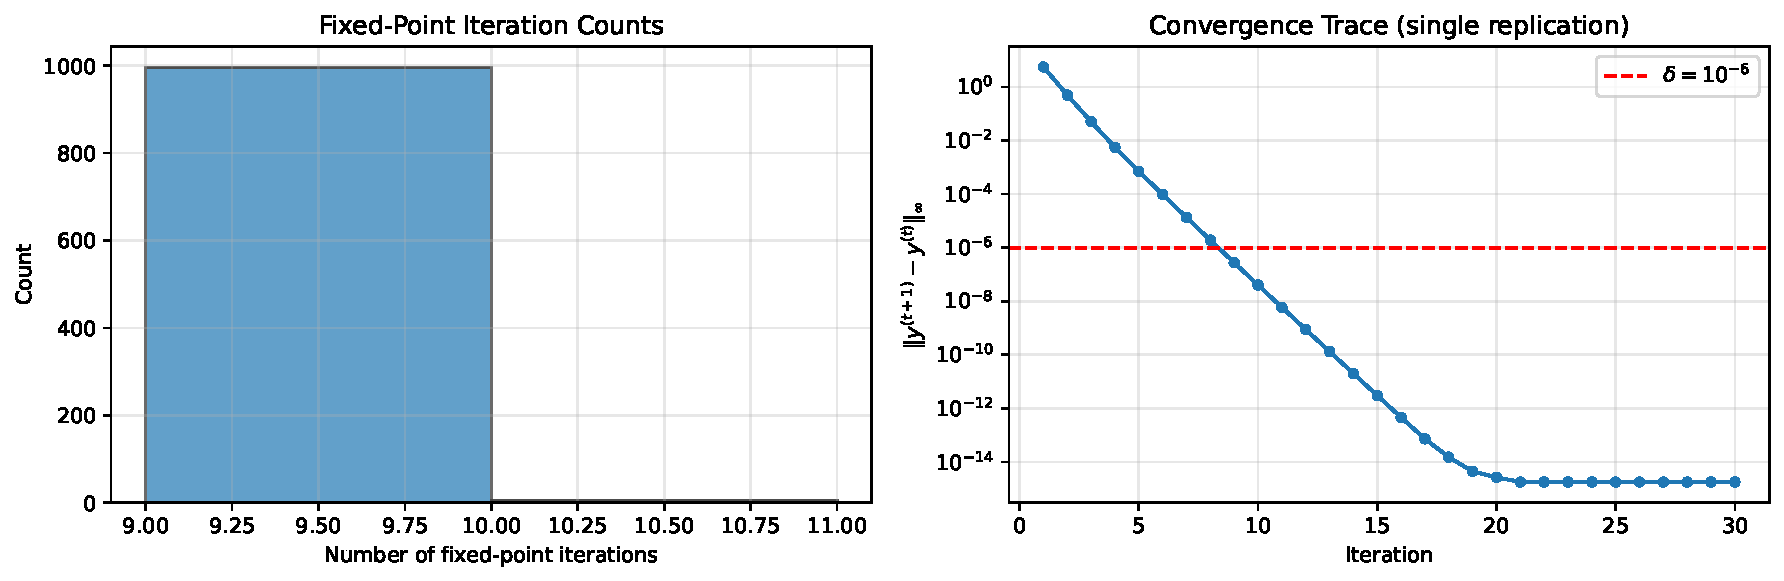
\includegraphics[width=\textwidth]{figures/mc_simul_fp_convergence.pdf}
    \caption[Fixed-point iteration convergence]{Visualisation of fixed-point iteration convergence across the $R = 1{,}000$ Monte Carlo replications. The left panel shows a histogram of the number of iterations to convergence with a tolerance of $\delta = 10^{-6}$. The right panel shows the geometric decrease in the maximum absolute change $\|\vect{y}^{(t+1)} - \vect{y}^{(t)}\|_\infty$ on a logarithmic scale, for a random replication.}
    \label{fig:mc_simul_fp_convergence}
\end{figure}

\begin{table}[htbp]
\centering
\caption[Monte Carlo results for FIML estimator of the simultaneous CoMO model]{Monte Carlo results for FIML estimator of the simultaneous CoMO model ($n = 500$, $R = 1{,}000$).}
\label{tab:mc_simul_results}
\begin{tabular}{lcccccc}
\toprule
Parameter & True & Mean Est. & Bias & Std(Est.) & Mean SE & Coverage \\
\midrule
$\beta_0$ & 3.50 & 3.4675 & $-0.0325$ & 0.8554 & 0.8274 & 0.952 \\
$\beta_1$ & 0.35 & 0.3483 & $-0.0017$ & 0.0778 & 0.0772 & 0.960 \\
$\beta_2$ & $-0.15$ & $-0.1437$ & 0.0063 & 0.1017 & 0.0970 & 0.938 \\
$\gamma_0$ & 7.00 & 7.0404 & 0.0404 & 0.6088 & 0.6027 & 0.951 \\
$\gamma_1$ & $-0.50$ & $-0.5027$ & $-0.0027$ & 0.0832 & 0.0823 & 0.943 \\
$\gamma_2$ & $-0.80$ & $-0.7998$ & 0.0002 & 0.0943 & 0.0946 & 0.952 \\
$\gamma_3$ & 0.25 & 0.2453 & $-0.0047$ & 0.0626 & 0.0627 & 0.942 \\
$\sigma_u^2$ & 1.44 & 1.4441 & 0.0041 & 0.1031 & 0.1023 & 0.951 \\
$\sigma_\varepsilon^2$ & 1.00 & 1.0008 & 0.0008 & 0.0677 & 0.0697 & 0.962 \\
\bottomrule
\end{tabular}
\end{table}

The mean estimates and biases show that the FIML estimator is approximately unbiased for all nine parameters. The largest bias is $0.040$ for $\gamma_0$, with $\beta_0$ also showing higher bias than the other parameters. We point to the discussion in Section~\ref{sec:mc:ml_screen} for why the intercepts have slightly higher bias and also why they have higher standard errors. We note that this is unproblematic and that the biases are still low. The Std(Est.) and Mean SE values are in close agreement for all parameters, and coverage is also close to the nominal 95\% across the board. This indicates that the standard errors based on the numerical Hessian are well-calibrated, and correctly capture the true sampling variability.

The coverages of $93.8\%$ for $\beta_2$ and $96.2\%$ for $\sigma_\varepsilon^2$ are the furthest from the nominal $95\%$. However, the Monte Carlo standard error for a $95\%$ coverage rate is approximately $\sqrt{0.95 \times 0.05/1{,}000} \approx 0.69$ percentage points when $R = 1{,}000$. Thus, $93.8\%$ and $96.2\%$ are about $1.7$ Monte Carlo standard errors from the nominal level, which is only a mild deviation.

In Figure~\ref{fig:mc_simul_hist_fiml} we plot histograms for estimates of all parameters. This gives a visual confirmation that the distributions of estimates are approximately symmetric and centred on the true values.

\begin{figure}[htbp]
    \centering
    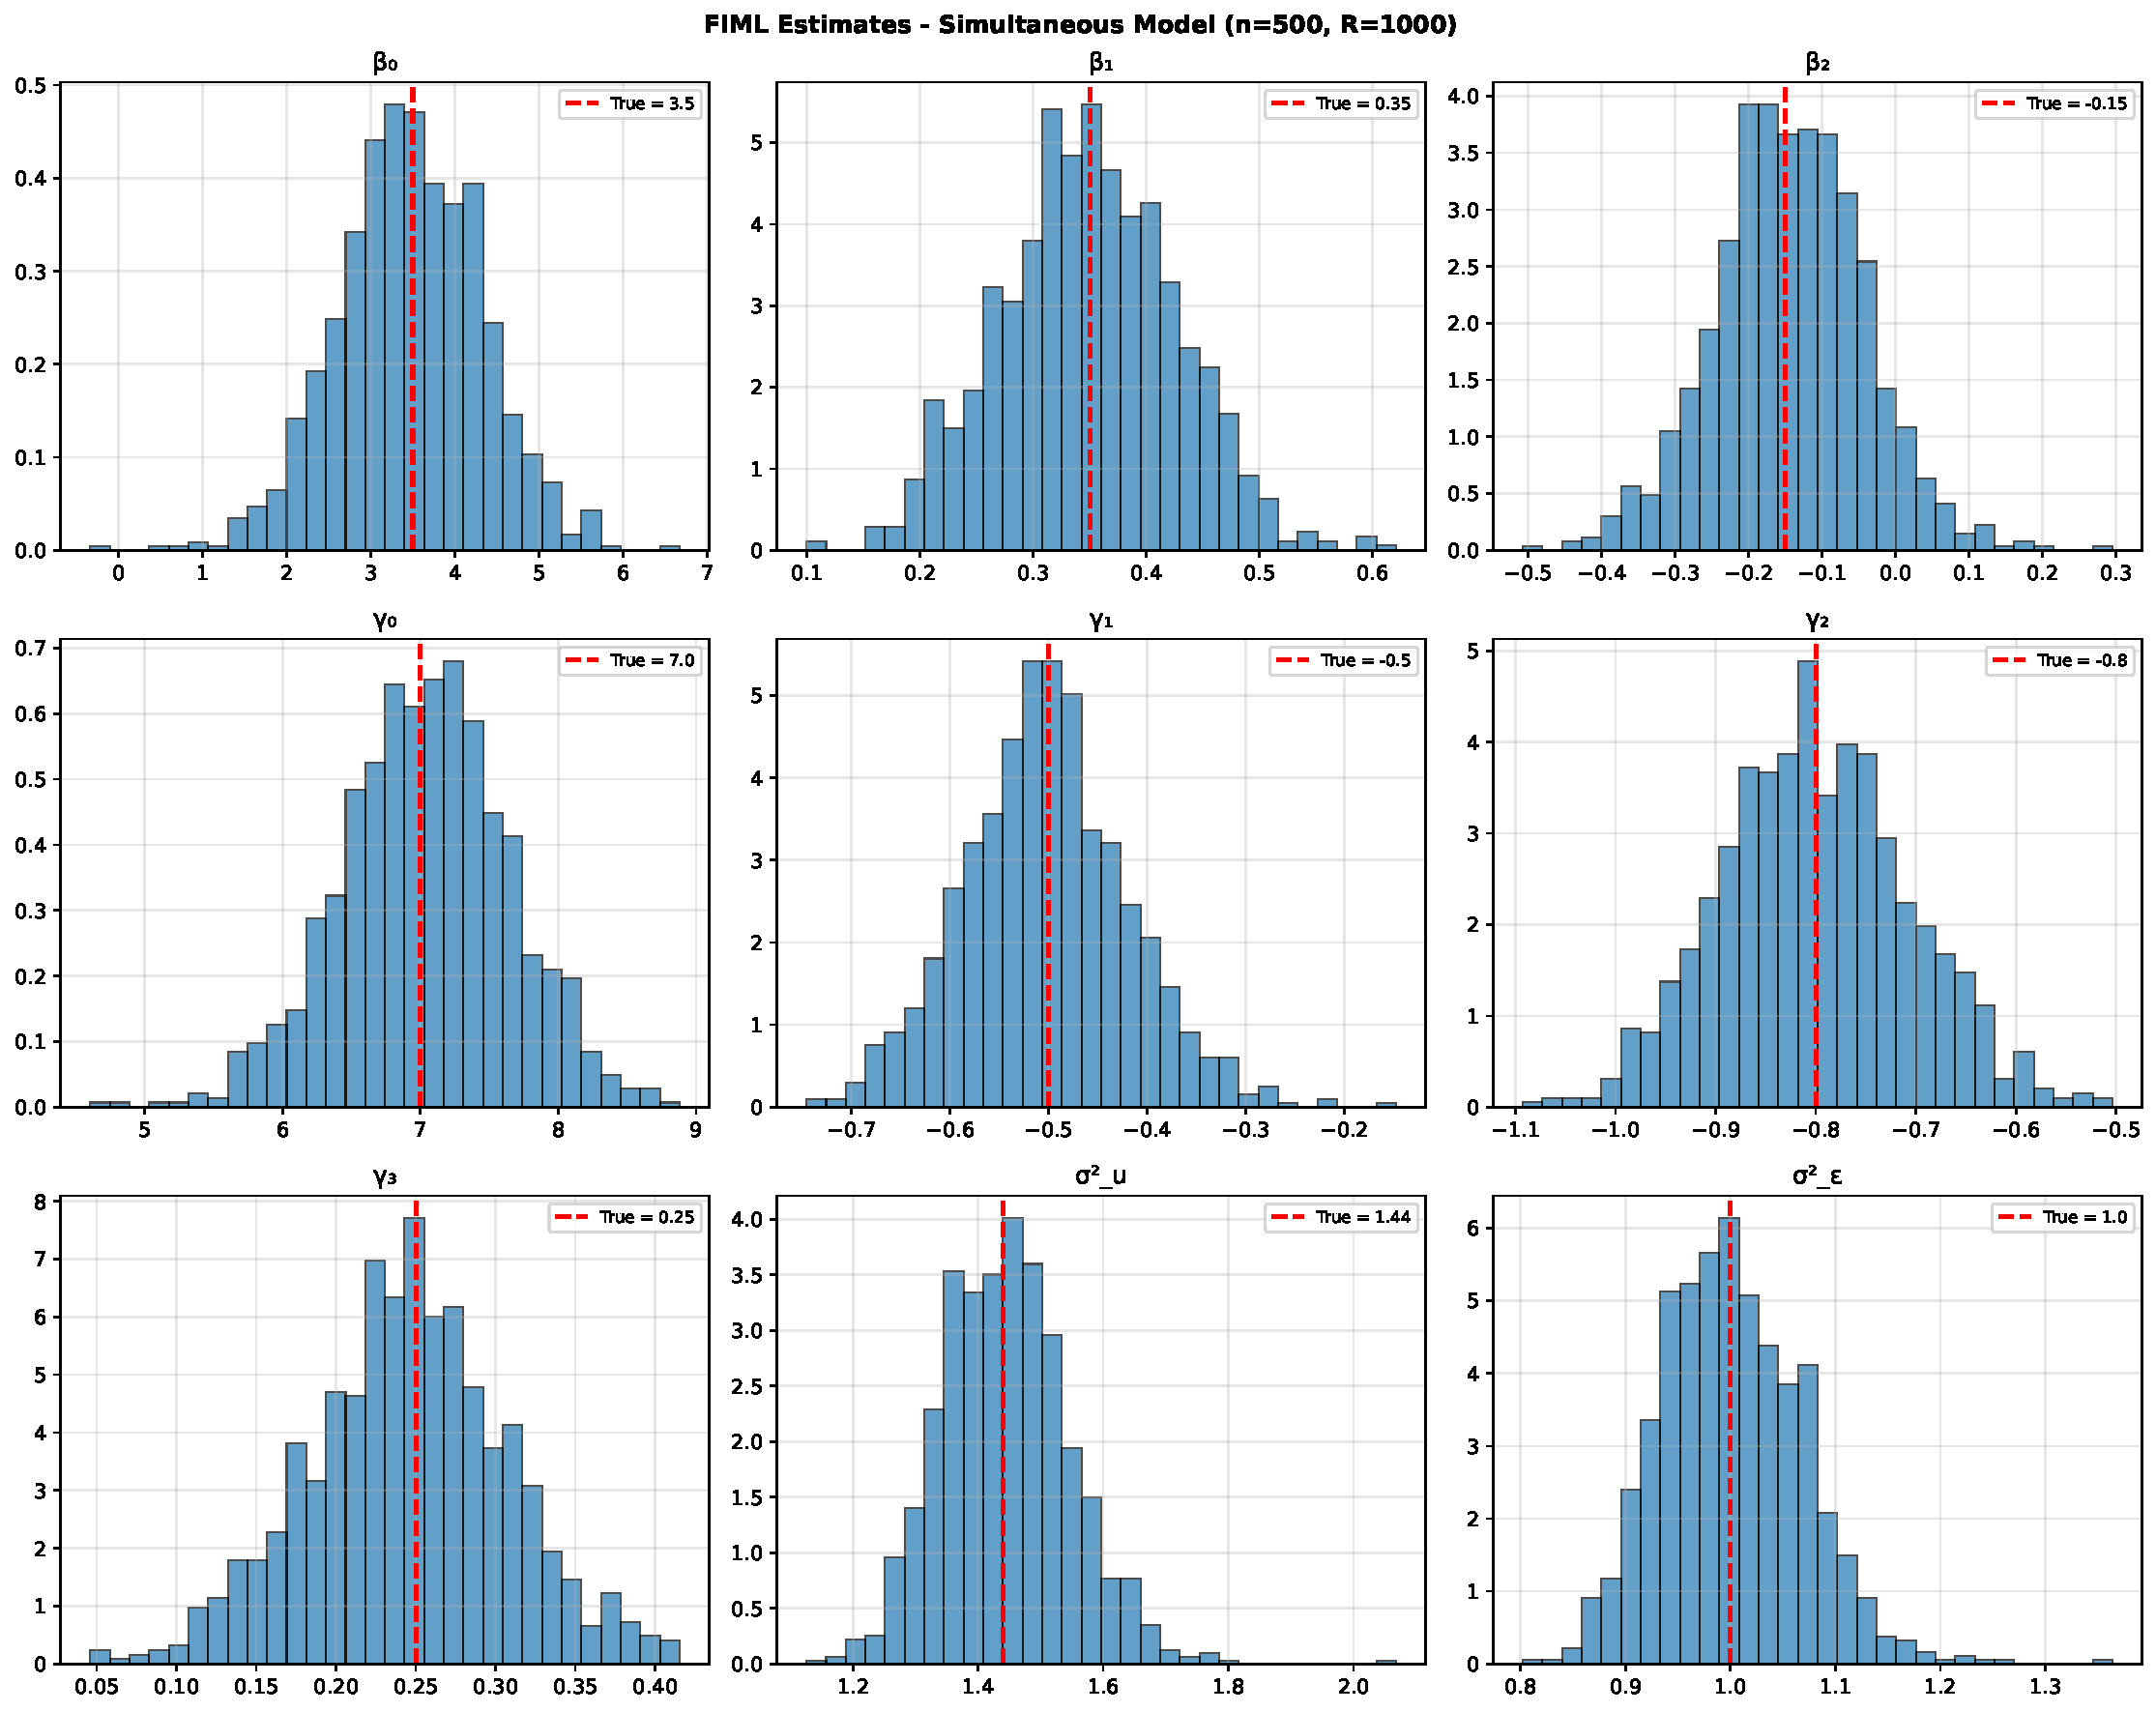
\includegraphics[width=\textwidth]{figures/mc_simul_hist_fiml.pdf}
    \caption[Histograms of FIML estimates]{The histograms display the FIML estimates for all nine parameters across the $R = 1{,}000$ Monte Carlo replications. The true parameter values are marked by red dashed lines. The histograms show approximate unbiasedness of the FIML estimators as the distributions are centred near the true values.}
    \label{fig:mc_simul_hist_fiml}
\end{figure}

\subsection{Assessment of Standard Errors}
\label{sec:simul:mc_se}
We now further assess the standard errors calculated by the numerical Hessian approximation. We do this through examining $z$-scores, and also through rejection rates from Wald tests of $H_0: \theta_k = \theta_k^0$, with $\theta_k^0$ the true parameter value. Under correct calibration of standard errors we expect the $z$-scores to be approximately standard normally distributed, and the empirical rejection rates at the $5\%$ level to be close to $0.05$.

This is exactly what we see. The results of the Wald tests are reported in Table~\ref{tab:mc_simul_rejection}, and show rejection rates hovering around the nominal 0.05 level. As in the analysis of Chapter~\ref{chap:monte_carlo}, we plot histograms of FIML $z$-scores in Figure~\ref{fig:mc_simul_zscore_hist}, and provide summary statistics in Table~\ref{tab:mc_simul_zscores}. Both the figure and summary statistics provide further evidence of proper calibration of Hessian-based standard errors: the $z$-scores are approximately standard normally distributed. All means are within $0.11$ of zero, and all standard deviations are within $0.04$ of one. Lastly, the values of skewness and kurtosis are small, with the largest in magnitude being $-0.292$ for skewness and $-0.271$ for kurtosis. These results correspond well with the coverages of Table~\ref{tab:mc_simul_results}, and confirm that the numerical Hessian-based standard errors are well-calibrated.

\begin{table}[htbp]
\centering
\caption[Empirical rejection rates for FIML Wald tests]{Empirical rejection rates at the $5\%$ level for FIML Wald tests ($n = 500$, $R = 1{,}000$, nominal: 0.05). Calculated as the Type I error rate under the null hypothesis that each parameter equals its true value.}
\label{tab:mc_simul_rejection}
\begin{tabular}{lc}
\toprule
Parameter & Rejection Rate \\
\midrule
$\beta_0$ & 0.048 \\
$\beta_1$ & 0.040 \\
$\beta_2$ & 0.062 \\
$\gamma_0$ & 0.049 \\
$\gamma_1$ & 0.057 \\
$\gamma_2$ & 0.048 \\
$\gamma_3$ & 0.058 \\
$\sigma_u^2$ & 0.049 \\
$\sigma_\varepsilon^2$ & 0.038 \\
\bottomrule
\end{tabular}
\end{table}

\begin{figure}[htbp]
    \centering
    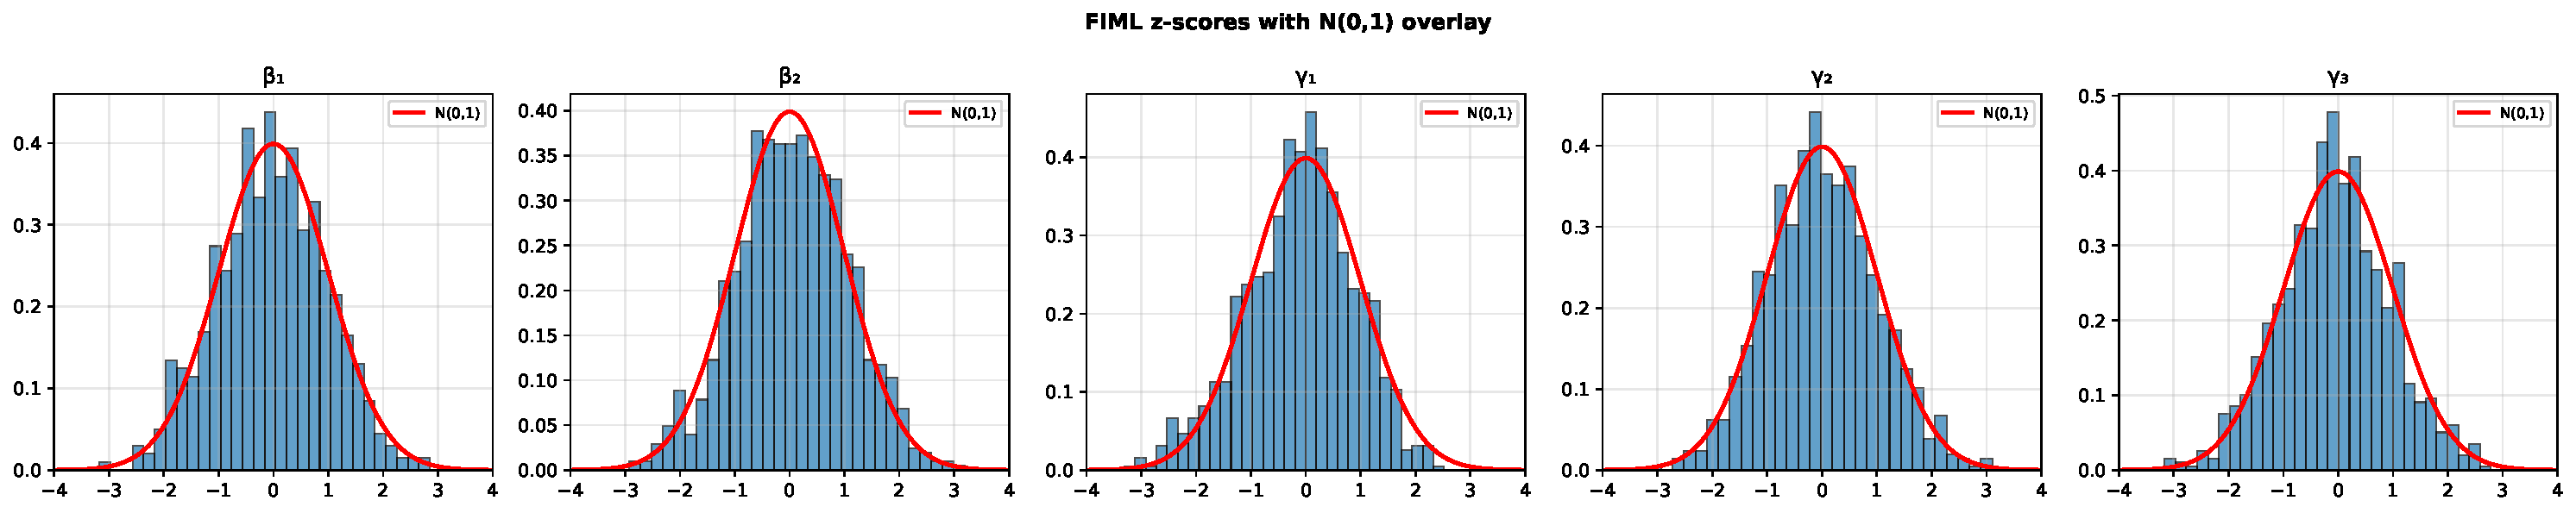
\includegraphics[width=\textwidth]{figures/mc_simul_zscore_hist.pdf}
    \caption[Histograms of FIML $z$-scores with $\N(0,1)$ overlays]{Histograms of FIML $z$-scores for the $R = 1{,}000$ Monte Carlo replications. Histograms are shown for the key parameters $\beta_1$, $\beta_2$, $\gamma_1$, $\gamma_2$, and $\gamma_3$. Red lines show overlays with $\N(0,1)$ densities. The approximate standard normal distribution of the $z$-scores signifies good calibration of the numerical Hessian-based standard errors.}
    \label{fig:mc_simul_zscore_hist}
\end{figure}

\begin{table}[htbp]
\centering
\caption[Summary statistics of FIML $z$-scores]{Summary statistics of FIML $z$-scores ($n = 500$, $R = 1{,}000$).}
\label{tab:mc_simul_zscores}
\begin{tabular}{lcccc}
\toprule
Parameter & Mean($z$) & Std($z$) & Skewness & Kurtosis \\
\midrule
$\beta_0$ & $-0.013$ & 1.002 & 0.061 & $-0.271$ \\
$\beta_1$ & $-0.037$ & 0.996 & $-0.041$ & $-0.257$ \\
$\beta_2$ & 0.054 & 1.018 & $-0.053$ & $-0.148$ \\
$\gamma_0$ & 0.110 & 1.000 & 0.186 & $-0.083$ \\
$\gamma_1$ & $-0.105$ & 0.997 & $-0.257$ & $-0.095$ \\
$\gamma_2$ & 0.003 & 0.994 & 0.099 & $-0.129$ \\
$\gamma_3$ & $-0.068$ & 0.999 & $-0.020$ & 0.018 \\
$\sigma_u^2$ & $-0.054$ & 1.007 & $-0.292$ & 0.240 \\
$\sigma_\varepsilon^2$ & $-0.084$ & 0.960 & $-0.240$ & $-0.124$ \\
\bottomrule
\end{tabular}
\end{table}

\subsection{Bias from Ignoring Feedback}
\label{sec:simul:mc_bias}
We now move on to testing the bias incurred when the recursive CoMO model (which assumes $\beta_2 = 0$) is used to estimate data generated from the simultaneous CoMO model ($\beta_2 = -0.15$). This is an important validation for the usefulness of the simultaneous CoMO model.

We generate data according to the DGP of the simultaneous CoMO model, using the parameters of Table~\ref{tab:mc_simul_params}, and then estimate parameters using both the FIML estimator and the now misspecified recursive ML estimators of Chapter~\ref{chap:estimation}. We report the results in Table~\ref{tab:mc_bias_comparison}. Here, $\beta_0$ and $\beta_2$ are omitted from the comparison. These are not comparable, as $\beta_2$ is not present in the recursive CoMO model, and $\beta_0$ has differing true values ($2.5$ in the recursive CoMO model, $3.5$ in the simultaneous CoMO model).

\begin{table}[htbp]
\centering
\caption[Bias comparison of recursive ML vs.\ FIML estimators]{Bias comparison of recursive ML vs.\ FIML estimators, fit on data from the simultaneous CoMO model ($n = 500$, $R = 1{,}000$). The FIML numbers are an independent Monte Carlo run, so there are small numerical differences from Table~\ref{tab:mc_simul_results} due to Monte Carlo sampling variability.}
\label{tab:mc_bias_comparison}
\begin{tabular}{lcccccccc}
\toprule
& & \multicolumn{3}{c}{Recursive ML} & \multicolumn{3}{c}{FIML} \\
\cmidrule(lr){3-5} \cmidrule(lr){6-8}
Parameter & True & Bias & Std(Est.) & RMSE & Bias & Std(Est.) & RMSE \\
\midrule
$\beta_1$ & 0.35 & 0.0735 & 0.0605 & 0.0952 & $-0.0034$ & 0.0772 & 0.0773 \\
$\gamma_0$ & 7.00 & 0.4106 & 0.4914 & 0.6404 & 0.0358 & 0.5872 & 0.5883 \\
$\gamma_1$ & $-0.50$ & $-0.0870$ & 0.0510 & 0.1009 & $-0.0003$ & 0.0816 & 0.0816 \\
$\gamma_2$ & $-0.80$ & 0.0304 & 0.0959 & 0.1006 & 0.0003 & 0.0959 & 0.0959 \\
$\gamma_3$ & 0.25 & $-0.0131$ & 0.0589 & 0.0603 & $-0.0057$ & 0.0604 & 0.0607 \\
$\sigma_u^2$ & 1.44 & 0.0736 & 0.1028 & 0.1265 & $-0.0025$ & 0.1040 & 0.1040 \\
$\sigma_\varepsilon^2$ & 1.00 & $-0.0218$ & 0.0623 & 0.0660 & 0.0012 & 0.0703 & 0.0704 \\
\bottomrule
\end{tabular}
\end{table}

The results show exactly what was expected: ignoring the feedback from WB to SMU biases the results of estimating with the recursive ML method on data from the simultaneous CoMO model. In particular, the recursive ML estimator exhibits a bias of $0.074$ in its estimation of $\beta_1$ (relative bias: $21\%$), and $0.411$ in the estimation of $\gamma_0$ (relative bias: $6\%$). Both biases are more than an order of magnitude higher than the FIML estimator equivalents. It also overestimates the magnitude of the direct SMU effect on WB ($\gamma_1$) by $0.087$. The recursive ML estimator for $\sigma_u^2$ also shows an upward bias of $0.074$ (relative bias: $5\%$). The FIML estimator, on the other hand, has negligible biases for all parameters.

The results can be explained by a misattribution occurring in the recursive ML estimator. When there is feedback from WB to SMU, we introduce a correlation between $\vect{s}$ and $\vect{\varepsilon}$. While the FIML estimator can account for this, the recursive ML estimator will misattribute this correlation. This can also be seen as a form of omitted-variable bias, as the omitted $\beta_2 y_i$ makes the effective error of the SMU equation $\tilde{u}_i = u_i + \beta_2 y_i$. This extra variation must be absorbed into the other regressors. For example, a negative WB shock ($\varepsilon_i < 0$) leads to a decrease in $y_i$ and corresponding increase in $s_i$ through $\beta_2$. This also raises $\sbar_j$, which inflates $\hat{\beta}_1$ even though there is no true increase in peer conformity. In this way the unmodelled feedback biases $\hat{\beta}_1$ from the recursive ML estimator. In the WB equation, $\vect{s}$ is endogenous as $s_i$ depends negatively on $\varepsilon_i$ through $\beta_2 y_i$. This negative correlation biases $\hat{\gamma}_1$ further away from zero. Lastly, the effective errors $\tilde{u}_i = u_i + \beta_2 y_i$ inflate the recursive ML estimate of $\sigma_u^2$, as it captures additional variance from the unmodelled feedback.

The RMSE values of the two models are quite closely aligned. Here there are two competing effects at play: a decrease in RMSE for the recursive CoMO model from fewer estimated parameters, and an increase in RMSE caused by biased estimates. For the parameters with the highest bias ($\beta_1$, $\gamma_0$, $\gamma_1$, $\sigma_u^2$), this leads to the FIML estimator having lower RMSE despite the additional parameter. Here, the largest difference is in $\sigma_u^2$, where the recursive RMSE is $22\%$ higher than the FIML RMSE ($0.127$ versus $0.104$). This corresponds to a relatively large difference in bias between the recursive and FIML estimates. However, for the parameters with lower bias ($\gamma_2$, $\gamma_3$, $\sigma_\varepsilon^2$), the RMSE values are approximately equal or lower for the recursive estimator.

\subsection{Size and Power of the Wald Test for Feedback}
\label{sec:simul:wald_test}
The nested nature of the recursive CoMO model within the simultaneous CoMO model (when $\beta_2 = 0$) allows us to test for the presence of feedback using a Wald test. This section assesses both the size of the test under $H_0: \beta_2 = 0$, and the power of the test against $\beta_2 = -0.15$. We also report numbers on the efficiency cost of using FIML over the recursive CoMO model.

We begin with the size of the test under the null hypothesis. We use the test statistic $z = \hat{\beta}_2 / \widehat{\text{SE}}(\hat\beta_2)$. Under $H_0$, this is approximately standard normally distributed. We run separate Monte Carlo simulations with the DGP of the recursive CoMO model ($\beta_0 = 2.5$, $\beta_2 = 0$, otherwise see Table~\ref{tab:mc_simul_params}), and $n = 500$ and $R = 1{,}000$ as before. Then, we estimate using the FIML model on this data. A rejection of this test signifies the presence of feedback from WB to SMU, implying a need for the simultaneous CoMO model. The results are presented in Table~\ref{tab:mc_wald_size}, and show that the test has approximately correct size. At all reported levels, the rejection rates are close to nominal. For the $5\%$ level, the discrepancy is the largest, with test rejections in $4.0\%$ of samples. However, with a Monte Carlo $95\%$ interval of $[3.6\%, 6.4\%]$, this is well within expected sampling variability.

\begin{table}[htbp]
\centering
\caption[Size of Wald test for $H_0: \beta_2 = 0$]{Size of Wald test for $H_0: \beta_2 = 0$ under $H_0$ ($n = 500$, $R = 1{,}000$).}
\label{tab:mc_wald_size}
\begin{tabular}{lc}
\toprule
Significance Level & Rejection Rate (Size) \\
\midrule
10\% & 0.092 \\
5\% & 0.040 \\
1\% & 0.011 \\
\bottomrule
\end{tabular}
\end{table}

This same simulation allows us to quantify the efficiency cost of using FIML when the DGP corresponds to the recursive CoMO model. We report the FIML standard deviations and mean SEs for the five shared parameters under the recursive DGP in Table~\ref{tab:mc_simul_efficiency}. We also include the corresponding values from the recursive ML simulation from Chapter~\ref{chap:monte_carlo}. The results show that there is increased variance in the sampling distributions of $\beta_1$, $\gamma_0$, and $\gamma_1$, which might be caused by the fact that FIML treats $\vect{s}$ as endogenous. The values for $\gamma_2$ and $\gamma_3$ are very similar for the two models. Coverage is close to nominal for all the parameters. We will discuss the practical implications of these results in Section~\ref{sec:simul:comparison}.

\begin{table}[htbp]
\centering
\caption[Efficiency cost of FIML vs.\ recursive estimators under the recursive DGP]{Comparison of efficiency cost of FIML and recursive CoMO estimators under the recursive CoMO DGP ($\beta_2 = 0$, $n = 500$, $R = 1{,}000$). The values for the recursive CoMO model are the same as in Tables~\ref{tab:mc_screen_ml} and~\ref{tab:mc_ml_results} of Chapter~\ref{chap:monte_carlo}.}
\label{tab:mc_simul_efficiency}
\begin{tabular}{lcccccc}
\toprule
& & \multicolumn{2}{c}{Recursive ML} & \multicolumn{3}{c}{FIML} \\
\cmidrule(lr){3-4} \cmidrule(lr){5-7}
Parameter & True & Std(Est.) & Mean SE & Std(Est.) & Mean SE & Coverage \\
\midrule
$\beta_1$    &  0.35 & 0.0646 & 0.0629 & 0.0779 & 0.0806 & 0.957 \\
$\gamma_0$   &  7.00 & 0.5050 & 0.5074 & 0.5658 & 0.5660 & 0.950 \\
$\gamma_1$   & $-0.50$ & 0.0538 & 0.0548 & 0.0848 & 0.0845 & 0.950 \\
$\gamma_2$   & $-0.80$ & 0.0938 & 0.0947 & 0.0976 & 0.0953 & 0.939 \\
$\gamma_3$   &  0.25 & 0.0623 & 0.0622 & 0.0630 & 0.0629 & 0.942 \\
\bottomrule
\end{tabular}
\end{table}

We now assess the empirical power of the test, investigating how often it correctly rejects $H_0$ when $\beta_2 = -0.15$. We use the main simulation design of this chapter with $\beta_2 = -0.15$. For each replication, we calculate the test statistic $z = \hat{\beta}_2 / \widehat{\text{SE}}(\hat\beta_2)$, and check whether $|z| > z_{1-\alpha/2}$ for each significance level. We note that one-sided tests could also be applied if warranted by prior knowledge, and that these would have increased power. The results of our simulations are reported in Table~\ref{tab:mc_wald_power}, and are the following: at the $10\%$, $5\%$, and $1\%$ levels, the rejection rates are $46.4\%$, $33.7\%$, and $15.1\%$, respectively. We also have that the mean test statistic is $\bar{z} = -1.52$, with $|\bar{z}| = 1.52$ below the two-sided $5\%$ critical value of $1.96$.

\begin{table}[htbp]
\centering
\caption[Power of Wald test for $H_0: \beta_2 = 0$ against $\beta_2 = -0.15$]{Power of Wald test for $H_0: \beta_2 = 0$ against $\beta_2 = -0.15$ ($n = 500$, $R = 1{,}000$).}
\label{tab:mc_wald_power}
\begin{tabular}{lc}
\toprule
Significance Level & Rejection Rate (Power) \\
\midrule
10\% & 0.464 \\
5\% & 0.337 \\
1\% & 0.151 \\
\bottomrule
\end{tabular}
\end{table}

These are moderate to low powers, which reflect the difficulty of detecting feedback (especially with low significance values) when we have $n = 500$ observations and an Erd\H{o}s--R\'enyi network with density $p = 0.01$. With this setup and the value $\beta_2 = -0.15$, the signal-to-noise ratio is too low for reliable detection in a single sample.

The unreliable detection can be verified through a direct calculation using $\widehat{\text{SE}}(\hat\beta_2) = 0.097$ from Table~\ref{tab:mc_simul_results}. Under the alternative, $z$ is approximately $\N(|\beta_2|/\widehat{\text{SE}}(\hat\beta_2), 1) \approx \N(1.55, 1)$, so the chance of $|z| > 1.96$ is approximately $\Phi(-0.41) \approx 0.34$. This matches the observed rejection rate of $33.7\%$ and $\bar z = -1.52$ closely.

The moderate power of $33.7\%$ at the $5\%$ level means that an application of the model to a single network dataset of $n = 500$ where true $\beta_2 = -0.15$ would fail to reject $H_0$ around two-thirds of the time. This is not due to any fault with the test, but is a consequence of the difficulty of the estimation problem. Whether or not the test rejects, we still retrieve unbiased estimates of all parameters when applying the FIML estimator. In practice, if the presence of feedback is in question, data can help answer the question by fitting the FIML estimator without introducing bias.

The results of the size and power of the Wald test show that the test is well-calibrated. It rejects at approximately nominal rates under $H_0$, and has expected moderate power. Larger sample sizes would increase the power. In practice, the test can be used to give information on whether or not the potential for feedback should be modelled. Including this in the model protects against the bias of an omitted variable, but reduces the efficiency of the estimator.

%% Section 7.4: Discussion
\section{Discussion}
\label{sec:simul:discussion}
This section briefly compares the recursive and simultaneous CoMO models, explains why we have not developed instrumental variables estimation for the simultaneous CoMO model, and discusses limitations and future work. This leads into the further discussion of Chapter~\ref{chap:discussion_conclusion}.

\subsection{Comparison of Recursive and Simultaneous CoMO Models}
\label{sec:simul:comparison}
Table~\ref{tab:recursive_vs_simul} provides an overview of the differences between the recursive and simultaneous CoMO models.

\begin{table}[htbp]
\centering
\caption[Comparison of recursive and simultaneous CoMO models]{Comparison of recursive and simultaneous CoMO models.}
\label{tab:recursive_vs_simul}
\small
\begin{tabular}{lcc}
\toprule
Feature & Recursive & Simultaneous \\
\midrule
Allows $y \to s$ feedback & No & Yes \\
Number of parameters & 8 & 9 \\
Closed-form reduced form & Yes & No (fixed-point) \\
ML estimation & Concentrated, 1D + 1D & Concentrated, 5D (warm-started) \\
Analytical Hessian & Derived (Chapter~\ref{chap:estimation}) & Not yet derived \\
Standard errors & Analytical & Numerical \\
IV identification & WB equation only & Not available (see Remark~\ref{rem:simul_no_iv}) \\
Monte Carlo validation & $R = 1{,}000$ (Ch.~\ref{chap:monte_carlo}) & $R = 1{,}000$ (this chapter) \\
\bottomrule
\end{tabular}
\end{table}

The simultaneous CoMO model introduces complexity through the $y \to s$ feedback, requiring the estimation of an additional parameter and increasing the dimensionality of the ML estimation. Instead of two one-dimensional optimisations, it requires solving a five-dimensional problem. It also introduces additional computational cost in the likelihood evaluations, which require a sparse log-determinant of the Schur complement. We also lack analytical standard errors and IV identification for comparison. This yields a trade-off between realism and robustness on the one hand, and computational cost on the other. If the feedback does exist, the simultaneous CoMO model does not exhibit omitted-variable bias (see Section~\ref{sec:simul:mc_bias}). If there is no such feedback, and the recursive CoMO model is true, estimating the simultaneous CoMO model is less efficient. This is because the model treats $\vect{s}$ as endogenous, which makes the sampling distributions of $\hat{\beta}_1$, $\hat{\gamma}_0$, and $\hat{\gamma}_1$ more variable (see Table~\ref{tab:mc_simul_efficiency}). The cost is most severe for the parameters $\beta_1$, $\gamma_0$, and $\gamma_1$, for which the FIML standard deviations are about $21\%$, $12\%$, and $58\%$ higher, respectively. For $\gamma_2$ and $\gamma_3$ the increases are small. However, coverage is still near $95\%$ for the FIML estimator even if the recursive CoMO model is true.

Using the FIML estimator also gives unbiased estimates, even when there is no feedback. Thus, in practice, if there is substantive uncertainty about whether feedback is present, fitting the FIML estimator as a robustness check can be worth it despite the efficiency cost. The Wald test for $H_0: \beta_2 = 0$ was shown to have moderate power when $n = 500$. While still providing information, non-rejection of the test is thus weak evidence for the absence of feedback. If there is good reason to believe that there is no feedback, or the efficiency gain is substantial, the recursive CoMO model is preferred.

\begin{remark}[Absence of IV Estimation]
\label{rem:simul_no_iv}
We include a remark on why IV estimation is not feasible for the simultaneous CoMO model in the current specification. For the recursive CoMO model, network instruments allowed for successful 2SLS estimation of the WB equation (see Section~\ref{sec:est:wb_2sls}). However, in the simultaneous CoMO model, the feedback makes all the non-intercept regressors endogenous. Both $\vect{s}$ and $\vect{c}(\vect{s})$ are correlated with the errors from the WB equation. This leaves us without any valid instruments usable for identification. In future work this could be addressed through the addition of exogenous individual-level covariates. This is similar to the SMU equation of the recursive CoMO model (see Section~\ref{sec:est:screen_2sls}). Instead of IV estimation, we thus only rely on the FIML approach, exploiting the distributional assumptions and the Jacobian structure for identification.
\end{remark}

\subsection{Limitations and Future Work}
\label{sec:simul:future}
We end the chapter with some limitations of the simultaneous CoMO model. These also provide directions for future work.

\begin{enumerate}
    \item \textbf{Analytical Hessian.} In our current implementation, standard errors are computed with a numerical Hessian approach requiring $O(p^2)$ likelihood evaluations. Both the speed and reliability of standard error computation could be improved by deriving the analytical Hessian of the FIML likelihood. Such a derivation would be algebraically involved, but is feasible in principle. This is left for future work.

    \item \textbf{Broader Monte Carlo validation.} In Chapter~\ref{chap:monte_carlo} we provided broad Monte Carlo validation of the recursive CoMO model estimators, investigating both the influence of varying sample sizes and network densities. This chapter provided an initial smaller Monte Carlo study with $R = 1{,}000$, which gave good evidence on both bias and coverage. However, a broader validation of the FIML estimator would strengthen confidence in it.

    \item \textbf{IV identification.} Remark~\ref{rem:simul_no_iv} discusses the lack of IV identification of the simultaneous CoMO model. Future work could develop IV estimators through extending the model with exogenous individual-level covariates. Exploring how the CoMO non-linearity could be exploited for identification is a different potential avenue for future research.

    \item \textbf{Sharper equilibrium conditions.} In Proposition~\ref{prop:contraction} we provided a sufficient condition for the Banach fixed-point theorem to guarantee the existence and uniqueness of the equilibrium. However, this constant~\eqref{eq:contraction_constant} is an upper bound that covers even the worst-case scenarios of operator norm estimates. Further work could sharpen this bound through, for example, exploiting spectral properties of the network $\mat{G}$, allowing for a stronger absolute influence of WB on SMU in the model.
\end{enumerate}

We have now developed the simultaneous CoMO model as well as the recursive specification of Chapter~\ref{chap:model}. This concludes the analytical framework of the thesis. In Chapter~\ref{chap:discussion_conclusion}, we return to the motivating research question, and combine these results with the ABM diagnosis of Chapter~\ref{chap:abm} to discuss the findings of the thesis.
